% Official competition template source:
% https://www.overleaf.com/read/vjztpvrnbrdh#43fbbe
\documentclass[sigconf]{acmart}
% Official competition template preamble, retained with minimal additions.
\setcopyright{none}
\settopmatter{printacmref=false}
\acmConference[Kaggle Competition]{Filament Segmentation Challenge}{2026}{\href{https://www.kaggle.com/competitions/filament-segmentation-2026}{kaggle.com/competitions/filament-segmentation-2026}}
\acmBooktitle{Competition Report}
\acmDOI{}
\acmISBN{}

\usepackage{xcolor}
\newif\ifguideStyle
\guideStyletrue
\newcommand{\guide}[1]{\ifguideStyle{\color{gray!65}\itshape #1}\fi}

\usepackage{mathtools}
\usepackage{subcaption}
\usepackage{tabularx}
\usepackage{multirow}


\guideStylefalse

\begin{document}

\title[High-Resolution Solar Filament Segmentation]{High-Resolution Solar Filament Instance Segmentation with Consensus Labels and Quality-Aware Calibration}
\subtitle{A Solution to the Solar Filament Segmentation Challenge 2026}

\author{CaoXin}
\authornote{Competition team: Cisdi Info Machine Vision Team.}
\affiliation{%
  \institution{CISDI Information Technology CO., LTD.}
  \city{Chongqing}
  \country{China}
}
\email{Xin.A.Cao@cisdi.com.cn}

\begin{abstract}
We present a reproducible instance-segmentation pipeline for GONG H-$\alpha$ observations.
YOLO26m-seg is trained at 2048-pixel resolution on 707 physical observations using
majority-consensus aggregation of repeated annotations. Our primary Y17-V system uses vertical-flip
test-time augmentation (TTA) and obtains two-fold out-of-fold Panoptic Quality (PQ) 0.4575.
QT01TTAH introduces a detached mask-IoU quality target and horizontal-flip TTA, obtaining PQ
0.4568. Both final candidates score 0.39 on the public leaderboard. Controlled ablations show that
candidate selection, rather than model capacity or raw proposal recall, is the main remaining
bottleneck.
\end{abstract}

\maketitle

% ==================================== %
%              INTRODUCTION            %
% ==================================== %
\section{Introduction}
This report goes over the details of our submitted solution to the Solar Filament Segmentation
Challenge~2026 \cite{filament-segmentation-2026}. The challenge, launched on July~10,~2026, is
organized by the Earth-Space AI Research (ESAIR) Lab\footnote{\href{https://www.esairlab.com/home}{www.esairlab.com/}}.
This challenge utilizes the MAGFiLO dataset for evaluation of the segmentation algorithms
\cite{ahmadzadeh2024dataset}. We target reliable instance recovery under low contrast, thin
morphology, and disagreement among repeated expert annotations. Our solution combines grouped
validation, consensus labels, high-resolution training, conservative flip TTA, and deterministic
non-overlapping output construction.

% ==================================== %
%              METHODOLOGY             %
% ==================================== %
\section{Methodology}\label{sec:methodology}

\subsection{Data representation and validation}
The released training set contains 707 physical observations; some have multiple independent
annotation passes. We keep every version of a physical observation in the same fold to prevent
leakage. Repeated passes are grouped into instance clusters by mask overlap, and an instance is
retained when supported by a majority of available passes. Each physical image is used once, so
observations with extra passes receive no additional optimization weight. The 145 two-pass images
have pairwise global PQ 0.3596 (559 TP, 476 FP, 393 FN), exposing substantial ambiguity. Expanding
consensus masks by union lowers Fold0/Fold1 PQ by 0.0207/0.0382, so we retain strict majority masks.

\begin{center}
  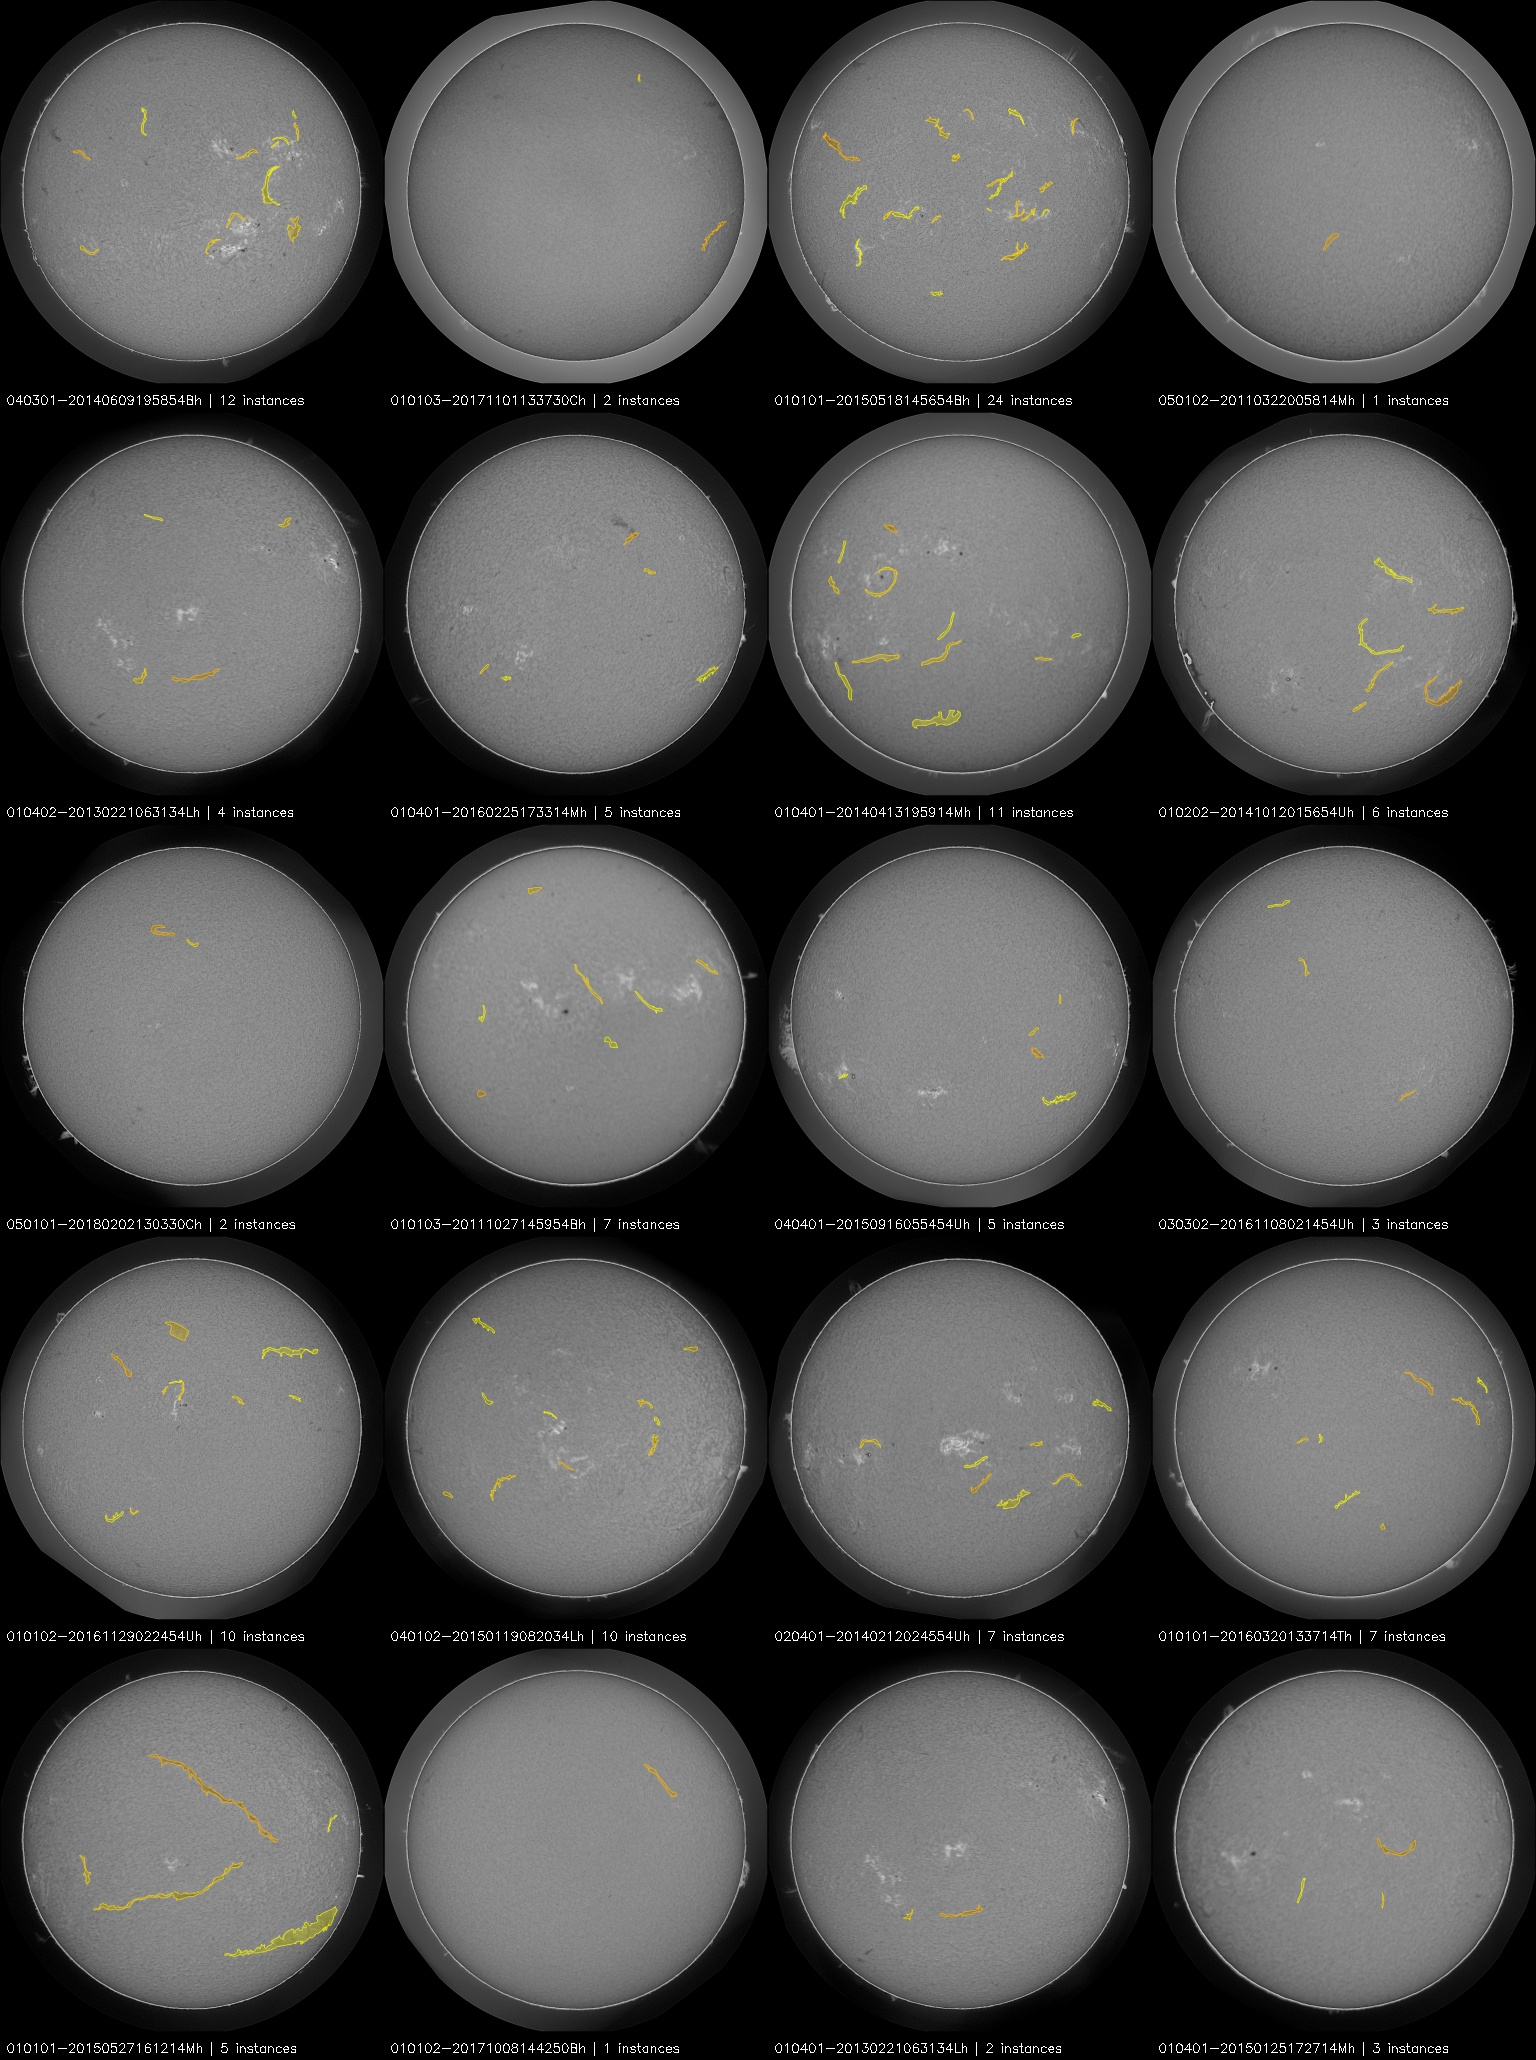
\includegraphics[width=.90\columnwidth,trim=0 1450 0 0,clip]{assets/annotation_diversity.jpg}
  \captionof{figure}{Training examples illustrate large variation in filament count, scale, contrast,
  and morphology. Colored contours show consensus instances.}
  \label{fig:diversity}
\end{center}

\begin{table}[!h]
\centering
\caption{Annotation controls and their implication.}
\label{tab:labels}
\small
\begin{tabularx}{\columnwidth}{lX}
\toprule
Control & Observation \\
\midrule
Two-pass agreement & Global PQ .3596; 559 TP, 476 FP, 393 FN \\
Strict majority & Best stable representation across both folds \\
Union expansion & Fold0/Fold1 PQ change $-.0207/-.0382$ \\
Random full pass & No public improvement over the .38 baseline \\
\bottomrule
\end{tabularx}
\end{table}

\subsection{Base model and training}
We initialize YOLO26m-seg \cite{ultralytics} from its official segmentation checkpoint and resize
images to $2048\!\times\!2048$. Mosaic, mixup, and copy-paste are disabled because they damaged
thin-structure continuity; mild rotation, translation, scale, intensity change, and flips remain.
Training uses seed 42, batch size 4, automatic mixed precision, and one NVIDIA RTX A6000. Raising
resolution from 1536 to 2048 improves Fold0 PQ from 0.4257 to 0.4342 and Fold1 from 0.4356 to
0.4620; public PQ rises from 0.37 to 0.38.

\begin{table}[!h]
\centering
\caption{Shared training configuration.}
\label{tab:training}
\small
\begin{tabular}{ll@{\qquad}ll}
\toprule
Item & Value & Item & Value \\
\midrule
Image size & 2048 & Batch & 4 \\
Seed & 42 & Precision & AMP \\
Mosaic & off & Mixup & off \\
Copy-paste & off & Max det. & 100 \\
\bottomrule
\end{tabular}
\end{table}

\begin{figure}[t]
  \centering
  \setlength{\fboxsep}{3pt}
  \small
  \fbox{Annotations $\rightarrow$ consensus instances $\rightarrow$ grouped folds}\\[3pt]
  $\Downarrow$\\[-1pt]
  \fbox{YOLO26m-seg @ 2048 $\rightarrow$ flip TTA $\rightarrow$ COCO RLE audit}
  \caption{End-to-end training, calibration, and submission pipeline.}
  \label{fig:pipeline}
\end{figure}

\subsection{Final systems}
\textbf{Y17-V.} The standard objective is trained on all 707 consensus observations for 22 epochs.
At inference, original and vertically flipped views are restored to common coordinates. Predictions
with mask IoU at least 0.50 are deduplicated by retaining the higher-confidence mask. The operating
point is confidence 0.28, minimum area 320 pixels, and at most 100 instances per image.

\textbf{QT01TTAH.} Classification confidence need not rank mask shape quality. For each assigned
positive, QT01 computes soft IoU between the predicted prototype mask and matched ground truth,
after cropping both to the target box, and uses
\begin{equation}
t_{QT}=0.5t_{TA}+0.5\,\operatorname{stopgrad}(\operatorname{IoU}_{mask}).
\end{equation}
Assignment, box, and mask losses are unchanged. The model is trained for 26 epochs and uses original
plus horizontal-flip inference, confidence 0.34, and minimum area 256 pixels.

\begin{table}[!h]
\centering
\caption{Frozen final inference settings.}
\label{tab:final-settings}
\small
\begin{tabular}{lcc}
\toprule
Setting & Y17-V & QT01TTAH \\
\midrule
Epochs & 22 & 26 \\
TTA views & original + V & original + H \\
Confidence & .28 & .34 \\
Minimum area & 320 & 256 \\
Duplicate IoU & .50 & .50 \\
Public PQ & .39 & .39 \\
\bottomrule
\end{tabular}
\end{table}

\subsection{Calibration and output construction}
Raw candidates are exported once at confidence 0.001, NMS IoU 0.70, and maximum 100 detections.
All sweeps reuse this cache. Y17 evaluates three flip modes; confidence .28, .32, .36, and .40; and
areas 256 and 320, selecting a setting only when it improves both folds. QT01 searches 12
confidences from .20 to .40 and areas 128, 256, 320, and 384 on Fold0; promotion requires
$\Delta$PQ$\geq.0108$, SQ regression $\leq.003$, and at most 50 additional false
positives. The selected point is frozen for Fold1 and full-data inference.

Candidates are processed by descending score. Pixels already assigned to a higher-scoring instance
are removed; area is recomputed; empty or sub-threshold masks are discarded and accepted masks are
COCO-RLE encoded. This deterministic procedure guarantees non-overlapping output instances.

\subsection{Metric-aligned operating-point selection}
The official metric can be factored as $\mathrm{PQ}=\mathrm{SQ}\times\mathrm{RQ}$, where SQ is the
mean IoU of matched instances and RQ penalizes both missed and spurious instances. Consequently, a
lower confidence threshold may increase recall while reducing PQ because every additional false
positive enlarges the denominator. Conversely, aggressive area filtering can improve apparent mask
cleanliness but convert weak true positives into false negatives. We therefore select operating
points using PQ, SQ, RQ, and TP/FP/FN jointly instead of mask loss or AP alone.

The cached-candidate workflow separates expensive neural inference from cheap deterministic
calibration. Each fold is inferred once at a permissive threshold; subsequent configurations only
decode masks, restore TTA coordinates, deduplicate, clip overlaps, and rerun the official matcher.
This makes every threshold comparison use an identical candidate pool and prevents GPU stochasticity
from being mistaken for a post-processing gain.

\begin{table}[!h]
\centering
\caption{Deterministic post-processing stages and their purpose.}
\label{tab:postprocess}
\small
\begin{tabularx}{\columnwidth}{lX}
\toprule
Stage & Function \\
\midrule
Restore & Map flip-view masks to original $2048^2$ coordinates \\
Filter & Apply frozen confidence and post-clip area thresholds \\
Deduplicate & Retain the higher score for mask IoU $\geq .50$ \\
Occupancy clip & Remove pixels owned by earlier, higher-scored instances \\
Audit & Decode RLE, check IDs, dimensions, overlap, and row count \\
\bottomrule
\end{tabularx}
\end{table}

% ==================================== %
%              EVALUATION              %
% ==================================== %
\section{Evaluation}\label{sec:evaluation}
We report official PQ \cite{kirillov2019panoptic}, Segmentation Quality (SQ), Recognition Quality
(RQ), and TP/FP/FN. Y17 uses cross-fold consistency over a predefined grid. QT01 selects on Fold0
and evaluates unchanged on Fold1, which acts as a frozen confirmation set. Public scores are never
used for calibration.

\begin{table}[t]
\centering
\caption{PQ of selected systems. Mean is over two grouped folds.}
\label{tab:main}
\small
\begin{tabular}{lcccc}
\toprule
Method & Fold0 & Fold1 & Mean & Public \\
\midrule
Y10/Y13 base & .4342 & .4620 & .4481 & .38 \\
Y17-V & .4430 & .4720 & \textbf{.4575} & \textbf{.39} \\
QT01TTAH & .4485 & .4651 & .4568 & \textbf{.39} \\
\bottomrule
\end{tabular}
\end{table}

Y17-V improves both matched base folds. QT01TTAH has comparable mean PQ while changing score
formation, making it a method-diverse second candidate. Y17-V emits 1,216 instances on 178/180 test
images; QT01TTAH emits 1,060 on 176/180. Both audited files contain valid $2048^2$ COCO RLE masks
and zero overlapping output pixels.

\subsection{Cross-fold and leaderboard interpretation}
The two folds differ by .0278 PQ for Y17-V and .0166 for QT01TTAH, which is material relative to most
ablation gains. We therefore reject changes supported by only one fold. Y17-V is the higher-mean,
standard-objective candidate; QT01TTAH is retained because it reaches the same public PQ through a
different confidence-learning mechanism and emits 156 fewer instances. The pair provides diversity
without using an unvalidated union that would increase false positives.

OOF means (.4575 and .4568) exceed public PQ (.39), but the ranking between the two systems remains
stable. We interpret this gap as evidence of distribution and annotation-policy differences, not as
a reason to tune on the public leaderboard. Final selection therefore combines grouped OOF PQ,
fold consistency, instance-count plausibility, qualitative morphology, and exact reproducibility.

\subsection{Ablations and error analysis}
Larger YOLO26l and alternative RF-DETR Seg, Mask2Former \cite{cheng2022mask2former}, EdgeCrafter,
and ConvNeXt-Tiny \cite{liu2022convnext} systems do not outperform YOLO26m. Unconditional ROI
refinement and topology repair regress. Tiled inference, difficult-image oversampling, disagreement
weighting, and instance SoftIoU also fail cross-fold confirmation. Figure~\ref{fig:ablation}
summarizes representative controls.

\begin{table}[!h]
\centering
\caption{Representative model-family comparison. Public PQ is used only as supporting evidence;
training budgets differ.}
\label{tab:model-family}
\small
\begin{tabular}{lc@{\qquad}lc}
\toprule
System & Public & System & Public \\
\midrule
RF-DETR R00 & .29 & EdgeCrafter E02 & .25 \\
EUPE ConvNeXt & .33 & Mask2Former & .37 \\
Selective refine & .37 & YOLO26m base & .38 \\
Y17-V & \textbf{.39} & QT01TTAH & \textbf{.39} \\
\bottomrule
\end{tabular}
\end{table}

\begin{center}
  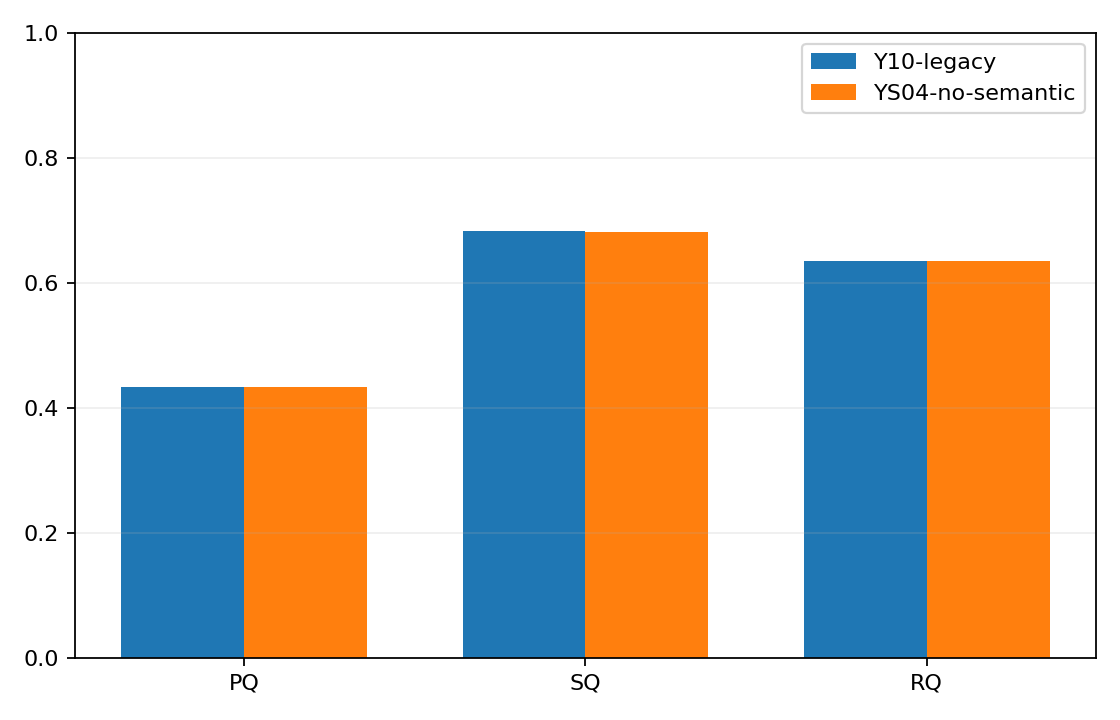
\includegraphics[width=.78\columnwidth]{assets/ablation_pq_sq_rq.png}
  \captionof{figure}{Representative local ablations evaluated with the official matcher.}
  \label{fig:ablation}
\end{center}

The semantic-head control in Figure~\ref{fig:counts} reduces false positives but loses more true
positives and increases false negatives, leaving PQ essentially unchanged. This illustrates why an
apparently cleaner mask output is not sufficient: PQ couples recognition and mask overlap.

\begin{center}
  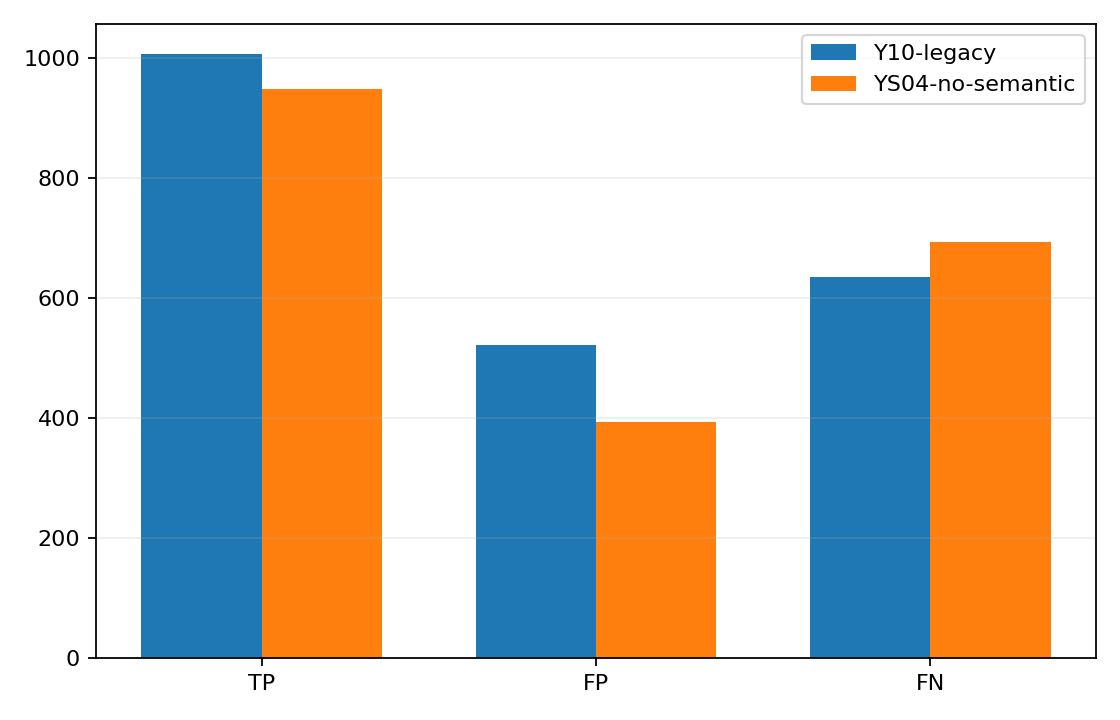
\includegraphics[width=.70\columnwidth]{assets/ablation_tp_fp_fn.png}
  \captionof{figure}{TP/FP/FN decomposition for the semantic-head control.}
  \label{fig:counts}
\end{center}

Candidates stored before final filtering cover 91.86\% of GT instances at IoU$>.5$, versus 62.09\%
after filtering. A GT-only fixed-count oracle reaches five-fold PQ 0.5737 versus approximately
0.4332; this is diagnostic and never used on test data. Yet global classifiers, pairwise rankers,
and visual verifiers yield only noise-level changes. Structured controls are likewise negative:
BD01 changes the two-fold mean from .4481 to .4441, XM01R changes it by $-.00064$, and CS01 is
negative on all five folds (mean $-.01944$). Candidate competition around the cutoff, not proposal
availability, is therefore the principal unresolved error source.

\begin{table}[!h]
\centering
\caption{Candidate-selection diagnostics. Oracle values are analysis only.}
\label{tab:candidates}
\small
\begin{tabular}{lr}
\toprule
Diagnostic & Result \\
\midrule
Raw candidates covering GT at IoU$>.5$ & 91.86\% \\
Final outputs covering GT at IoU$>.5$ & 62.09\% \\
Observed five-fold PQ & $\sim$.4332 \\
GT-only fixed-count oracle PQ & .5737 \\
BD01 / XM01R / CS01 mean change & $-.0040/-.00064/-.01944$ \\
\bottomrule
\end{tabular}
\end{table}

Qualitatively, both systems preserve elongated bodies and suppress many compact sunspot-like false
positives. Remaining errors are fully missed faint filaments, fragmented low-contrast boundaries,
and ambiguous instances caused by annotation disagreement. The limited sample and label ambiguity
make single-fold improvements unreliable.

\begin{center}
\begin{minipage}{.98\columnwidth}
  \centering
  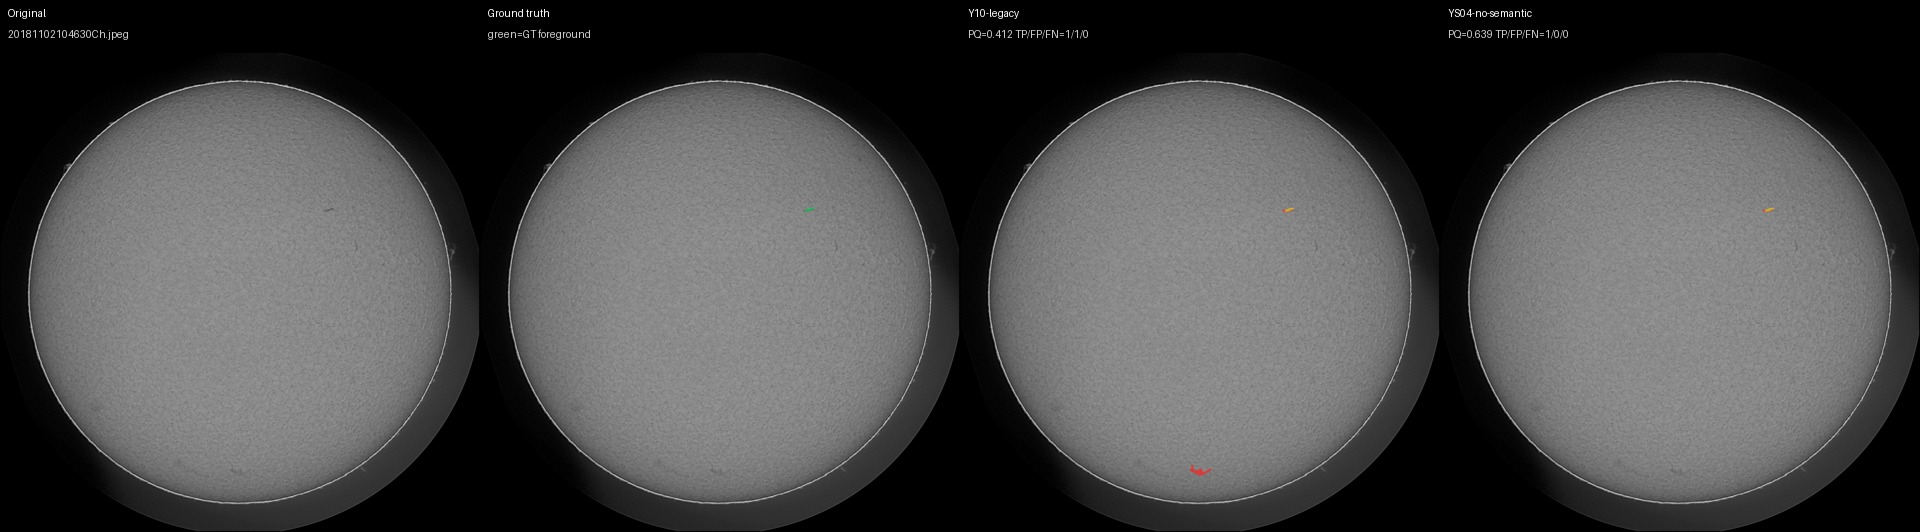
\includegraphics[width=.88\linewidth]{assets/qualitative_improved.jpg}\\[-1pt]
  \textbf{(a) Recovered/cleaner cases}\\[3pt]
  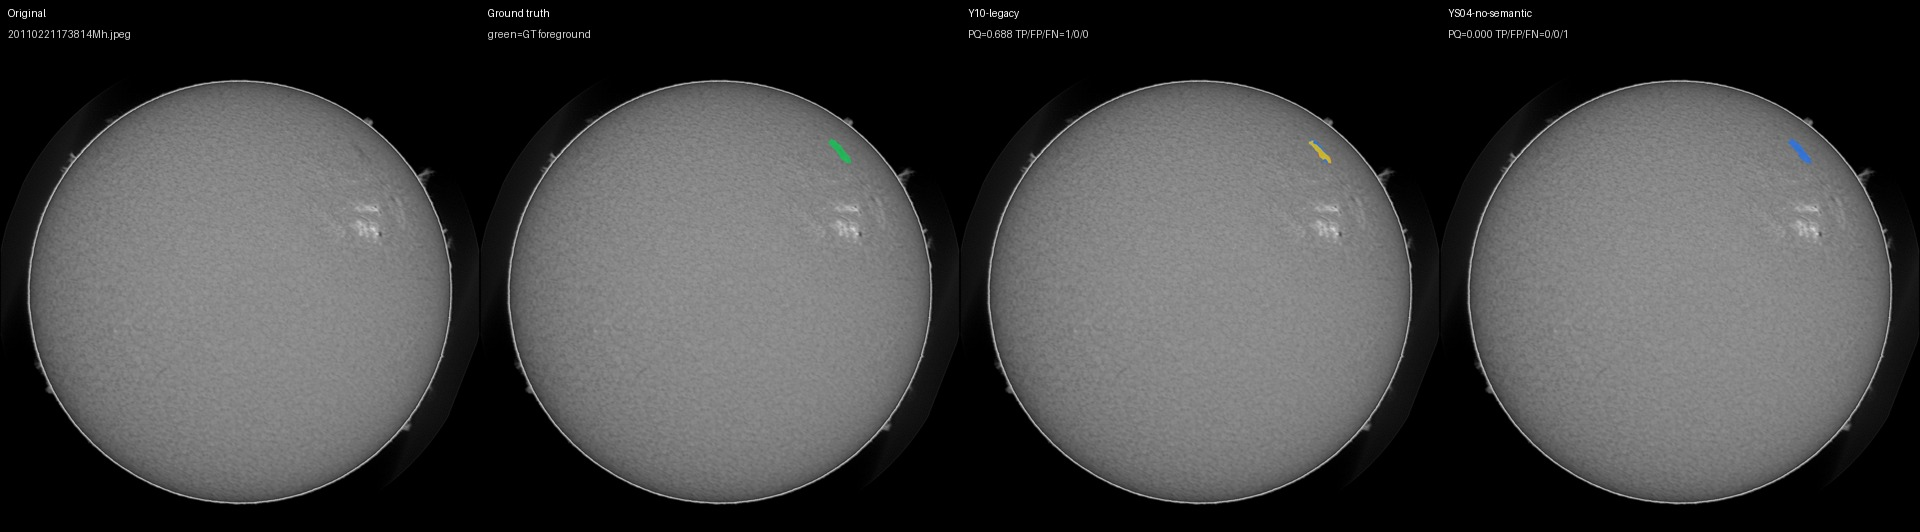
\includegraphics[width=.88\linewidth]{assets/qualitative_regressed.jpg}\\[-1pt]
  \textbf{(b) Remaining failures}
  \captionof{figure}{Representative validation predictions. Each strip shows the H-$\alpha$ image,
  reference, and model overlays generated by the evaluation script.}
  \label{fig:qualitative}
\end{minipage}
\end{center}

\begin{table}[!h]
\centering
\caption{Dominant failure modes and the corresponding control.}
\label{tab:failures}
\small
\begin{tabularx}{\columnwidth}{lX}
\toprule
Failure & Evidence or mitigation \\
\midrule
Weak-filament miss & TTA recovers some cases; lower thresholds add more FP than TP \\
Fragmentation & Static joining and topology repair regress PQ \\
Merged neighbors & Instance masks and occupancy clipping preserve separation \\
Sunspot-like FP & Confidence/area calibration is more stable than a learned verifier \\
Label ambiguity & Grouped folds and majority labels prevent leakage and overweighting \\
\bottomrule
\end{tabularx}
\end{table}

\subsection{Efficiency and reproducibility}
Table~\ref{tab:efficiency} reports measured end-to-end costs on one RTX A6000. Full-resolution mask
serialization and fusion, rather than model execution alone, dominate TTA latency.

\begin{table}[!h]
\centering
\caption{Measured resource and runtime profile.}
\label{tab:efficiency}
\small
\begin{tabular}{lr}
\toprule
Operation & Measured cost \\
\midrule
Y17, 22-epoch full training & 1.119 h \\
QT01, 26-epoch full training & 1 h 33 min 30 s \\
Peak training memory & $\sim$33.7 GB \\
Model-only validation inference & 52.5 ms/image \\
QT01 base test prediction, 180 images & 7 min 7 s \\
Extra H-flip export and fusion & 14 min 20 s \\
\bottomrule
\end{tabular}
\end{table}

The release includes pinned dependencies, exact configurations, consensus-label preparation,
training and inference entry points, a complete notebook, checkpoints, cached TTA predictions,
submission audits, and SHA256 manifests. The original checkpoints use the repository's
Ultralytics 8.4.3 checkout; the clean release pins 8.4.15 and reproduces archived CSV hashes. Only
competition training annotations are used; public MAGFiLO annotations corresponding to competition
test observations were neither accessed nor used.

Reproduction has two supported levels. Exact reconstruction starts from archived raw predictions
and deterministically rebuilds both CSV hashes; model reproduction downloads the released
checkpoints and reruns base/TTA inference. Full retraining additionally rebuilds consensus labels
from the official COCO JSON and trains from the declared pretrained checkpoint. The verification
script checks required files, SHA256 values, CSV columns, all test identifiers, RLE decodability,
mask dimensions, and the absence of overlapping output pixels. Competition data are intentionally
excluded from the public repository.

\begin{table}[!h]
\centering
\caption{Public reproduction artifacts.}
\label{tab:artifacts}
\small
\begin{tabularx}{\columnwidth}{lX}
\toprule
Artifact & Reproduction role \\
\midrule
Configurations & Freeze training, TTA, thresholds, and area filters \\
Notebook & Execute preparation through audited submission generation \\
Checkpoints & Reproduce model inference for both final candidates \\
Raw predictions & Rebuild exact CSV files without retraining \\
Manifest/SHA256 & Verify provenance and byte-level identity \\
\bottomrule
\end{tabularx}
\end{table}

\subsection{Conclusion}
High-resolution YOLO26m with conservative flip TTA is the most reliable configuration.
Quality-aware targets provide a competitive alternative, but both candidates plateau at public PQ
0.39. Future work should prioritize set-aware candidate ranking and conservative matched-instance
mask selection rather than simply increasing capacity or proposal count.

% ==================================== %
%            ACKNOWLEDGMENT            %
% ==================================== %
\section{Acknowledgment}\label{sec:acknowledgment}
The organization of the Filament Segmentation Challenge 2026 is partially supported by the U.S.
National Science Foundation (NSF) under Grant No. 2209912 and 2433781, directorate for Computer and
Information Science and Engineering (CSE), and Office of Advanced Cyberinfrastructure (OAC), and
Grant No. 2511630, AST Division Of Astronomical Sciences and MPS Directorate for Mathematical and
Physical Sciences.

The Filament Segmentation Challenge 2026 is sponsored by the U.S. National Science Foundation
(NSF) National Solar Observatory (NSO).

This work utilizes GONG data obtained by the NSO Integrated Synoptic Program, managed by the
National Solar Observatory, which is operated by the Association of Universities for Research in
Astronomy (AURA), Inc. under a cooperative agreement with the National Science Foundation and with
contribution from the National Oceanic and Atmospheric Administration. The GONG network of
instruments is hosted by the Big Bear Solar Observatory, High Altitude Observatory, Learmonth Solar
Observatory, Udaipur Solar Observatory, Instituto de Astrof\'isica de Canarias, and Cerro Tololo
Interamerican Observatory.

\bibliographystyle{ACM-Reference-Format}
\bibliography{main}

\end{document}
